\documentclass[11pt,a4paper]{amsart}

%% ─── Encoding & language ───────────────────────────────────────────
\usepackage[T1]{fontenc}
\usepackage[utf8]{inputenc}
\usepackage[english]{babel}

%% ─── Typography ────────────────────────────────────────────────────
\usepackage{microtype}
\usepackage{csquotes}

%% ─── Mathematics ───────────────────────────────────────────────────
\usepackage{amsmath, amssymb, amsthm}
\numberwithin{equation}{section}

%% ─── Page layout ───────────────────────────────────────────────────
\raggedbottom

%% ─── Lists, tables, figures & algorithms ──────────────────────────
\usepackage{enumitem}
\usepackage{booktabs}
\usepackage{graphicx}
\graphicspath{{project/figures/}}
\usepackage{algorithm}
\usepackage[noend]{algpseudocode}

%% ─── Bibliography ──────────────────────────────────────────────────
\usepackage[
  backend=biber,
  style=numeric-comp,
  sorting=none,
  giveninits=true,
  doi=true,
  url=false,
  isbn=false,
  eprint=true,
  maxbibnames=99,
  maxcitenames=2
]{biblatex}
\addbibresource{seminar.bib}
\AtEveryBibitem{\clearlist{language}}
\renewcommand*{\bibfont}{\normalfont\footnotesize}  % amsart's \bibliofont
\renewcommand*{\postnotedelim}{\addcomma\addnbspace}

%% ─── Hyperlinks & metadata ─────────────────────────────────────────
\usepackage{hyperref}
\hypersetup{
  colorlinks=true,
  linkcolor=black,
  citecolor=blue,
  urlcolor=blue,
  pdftitle={The BFGS and L-BFGS Methods},
  pdfauthor={Elvir Muslić}
}
\usepackage{orcidlink}

%% ─── Theorem environments ─────────────────────────────────────────
\theoremstyle{plain}
\newtheorem{theorem}{Theorem}[section]
\newtheorem{proposition}[theorem]{Proposition}
\newtheorem{lemma}[theorem]{Lemma}
\newtheorem{corollary}[theorem]{Corollary}

\theoremstyle{definition}
\newtheorem{definition}[theorem]{Definition}
\newtheorem{example}[theorem]{Example}

\theoremstyle{remark}
\newtheorem{remark}[theorem]{Remark}

%% ─── Algorithms ───────────────────────────────────────────────────
\algrenewcommand\algorithmicrequire{\textbf{Input:}}
\algnewcommand{\IfThen}[2]{\State \algorithmicif\ #1\ \algorithmicthen\ #2}
\algnewcommand{\ElsIfThen}[2]{%
  \State \algorithmicelse\ \algorithmicif\ #1\ \algorithmicthen\ #2}
\algnewcommand{\ElseDo}[1]{\State \algorithmicelse\ #1}

%% ─── Notation shortcuts ───────────────────────────────────────────
\newcommand{\R}{\mathbb{R}}
\newcommand{\grad}{\nabla}
\newcommand{\T}{\mathsf{T}}
\newcommand{\norm}[1]{\lVert #1 \rVert}
\newcommand{\code}[1]{\texttt{#1}}

\begin{document}

%% ─── Seminar cover page ───────────────────────────────────────────
\thispagestyle{empty}
\begin{center}
  {\large University of Niš\par}
  {\large Faculty of Sciences and Mathematics\par}
  \smallskip
  Department of Computer Science\par
  Doctoral Academic Studies in Computer Science\par

  \vspace{3em}
  {\itshape Seminar paper\par}
  {\itshape Course: Advanced Numerical Optimization (20.IDI16)\par}

  \vspace{3.5em}
  \rule{\linewidth}{0.4pt}\par
  \vspace{1em}
  {\LARGE\bfseries The BFGS and L-BFGS Methods\par}
  \vspace{1em}
  \rule{\linewidth}{0.4pt}\par
\end{center}

\vspace{3.5em}
\noindent
\begin{minipage}[t]{0.49\linewidth}
  \raggedright
  \textbf{Mentor}\par
  Prof.\ Marko Miladinović
\end{minipage}\hfill
\begin{minipage}[t]{0.49\linewidth}
  \raggedleft
  \textbf{Student}\par
  Elvir Muslić\,\orcidlink{0009-0006-4042-6550}\par
  ORCID \href{https://orcid.org/0009-0006-4042-6550}{0009-0006-4042-6550}
\end{minipage}

\vfill
\begin{center}Niš, October 2026\end{center}
\newpage

%% ─── Abstract & front information ─────────────────────────────────
\begin{center}\scshape Abstract\end{center}
\noindent
Quasi-Newton methods minimize a smooth function of $n$ variables without
second derivatives: after every step, they correct an approximation of
the inverse Hessian from the change of the gradient. This paper
motivates the BFGS update by the secant equation, proves that it stays
positive definite under the strong Wolfe conditions, and presents a line
search for these conditions, the limited-memory variant L-BFGS with its
two-loop recursion, and four convergence results. Our own
implementations of gradient descent, BFGS and L-BFGS are compared on the
Rosenbrock function and two test functions with up to $10^6$ variables,
with SciPy only as a check. On the Rosenbrock function, BFGS
needs $38$ iterations and gradient descent $5508$. With five stored
pairs, L-BFGS solves both test functions at $n = 10^6$, in $1104$ and
$239$ iterations. Along SciPy's steps, our update reproduces SciPy's
BFGS matrix to a relative difference of $3.0 \cdot 10^{-13}$.

\bigskip
\setcounter{tocdepth}{1}
\tableofcontents

%% ═══════════════════════════════════════════════════════════════════
\section{Introduction}\label{sec:intro}

This paper is about the unconstrained problem
\begin{equation}\label{eq:problem}
  \min_{x \in \R^n} f(x),
\end{equation}
where $f : \R^n \to \R$ is twice continuously differentiable. In words,
\eqref{eq:problem} asks for a point $x^*$ at which $f$ is smallest.

Newton's method steps to the minimizer of the second-order Taylor model
of $f$ at $x_k$, $p_k = -\grad^2 f(x_k)^{-1} \grad f(x_k)$. Near a
minimizer with a positive definite, Lipschitz continuous Hessian it
converges quadratically~\cite[\S3.3]{nocedal2006}, but each step needs
$n(n+1)/2$ second derivatives and an $O(n^3)$ linear solve.

Quasi-Newton methods replace $\grad^2 f(x_k)^{-1}$ by a matrix $H_k$, so
that the direction $-H_k \grad f(x_k)$ costs one matrix-vector product,
$O(n^2)$ operations, instead of a linear solve. They correct $H_k$ after
each step from gradients alone, also in $O(n^2)$ operations, and still
converge superlinearly~\cite{dennis1977,nocedal2006,miladinovic2015}.
The best known is BFGS, by Broyden, Fletcher, Goldfarb and
Shanno~\cite{broyden1970,fletcher1970,goldfarb1970,shanno1970}. Its
limited-memory variant L-BFGS~\cite{nocedal1980,liu1989} stores a few
vectors, not $H_k$, and handles millions of variables. The paper does
four things.
\begin{enumerate}[leftmargin=*, nosep]
\item Section~\ref{sec:bfgs} presents the BFGS update, proves that it
  stays positive definite, and gives its algorithm.
\item Section~\ref{sec:lbfgs} derives L-BFGS and its two-loop recursion.
\item Section~\ref{sec:convergence} states four convergence results.
\item Section~\ref{sec:experiments} tests our code up to $n = 10^6$,
  checked against SciPy~\cite{scipy2020,byrd1995}.
\end{enumerate}

%% ═══════════════════════════════════════════════════════════════════
\section{The BFGS Method}\label{sec:bfgs}

\subsection{The secant condition}\label{sec:secant}

Write $g_k = \grad f(x_k)$; $\norm{\cdot}$ is the Euclidean norm. A line
search method moves from $x_k$ along a direction $p_k$ by a step length
$\alpha_k > 0$, needed because the direction comes from a local model
that can mislead far from $x^*$. A quasi-Newton method uses the Newton
direction with $\grad^2 f(x_k)^{-1}$ replaced by a symmetric positive
definite matrix $H_k$:
\begin{equation}\label{eq:iteration}
  x_{k+1} = x_k + \alpha_k p_k, \qquad p_k = -H_k\, g_k .
\end{equation}
In words, the method moves along the negative gradient transformed by
$H_k$, by a distance set by $\alpha_k$; with $H_k = I$ it is gradient
descent. Since $g_k^\T p_k = -g_k^\T H_k g_k < 0$ for $g_k \neq 0$,
$p_k$ is a \emph{descent direction}: the slope of $f$ along $p_k$ is
negative, so $f$ decreases for small enough $\alpha_k$.

The step length must decrease $f$ enough, and it must not be too short,
since tiny steps can decrease $f$ at every iteration and still stall far
from $x^*$. For constants $0 < c_1 < c_2 < 1$, the \emph{strong Wolfe
conditions}~\cite[(3.7)]{nocedal2006} are
\begin{align}
  f(x_k + \alpha_k p_k) &\leq f(x_k) + c_1\, \alpha_k\, g_k^\T p_k,
    \label{eq:armijo}\\
  \bigl\lvert \grad f(x_k + \alpha_k p_k)^\T p_k \bigr\rvert
    &\leq c_2\, \bigl\lvert g_k^\T p_k \bigr\rvert .
    \label{eq:wolfe}
\end{align}
In words, the \emph{sufficient decrease condition}~\eqref{eq:armijo}
asks for at least a fraction $c_1$ of the decrease promised by the slope
$g_k^\T p_k$, and the \emph{strong curvature condition}~\eqref{eq:wolfe}
asks the slope along $p_k$ to shrink to at most a fraction $c_2$ of its
initial size, so that $f$ neither still falls nor already rises steeply
where the step ends. We use $c_1 = 10^{-4}$ and $c_2 = 0.9$, the usual
values for quasi-Newton methods~\cite[Ch.~3]{nocedal2006}.

The Hessian is not available, but each step reveals curvature through
the pair
\begin{equation}\label{eq:sy}
  s_k = x_{k+1} - x_k = \alpha_k p_k, \qquad y_k = g_{k+1} - g_k .
\end{equation}
In words, $s_k$ is the step just taken and $y_k$ the change of the
gradient over it. By Taylor's theorem,
$y_k = \grad^2 f(x_{k+1})\, s_k + o(\norm{s_k})$, and $y_k = A s_k$
exactly for a quadratic with Hessian $A$. Asking the new matrix to
reproduce this relation gives the \emph{secant equation}, also called
the secant condition,
\begin{equation}\label{eq:secant}
  H_{k+1}\, y_k = s_k .
\end{equation}
In words, $H_{k+1}$ must map the observed change of the gradient back to
the step that caused it, as the inverse Hessian of a quadratic does.

A positive definite $H_{k+1}$ can satisfy~\eqref{eq:secant} only if
$y_k^\T s_k = y_k^\T H_{k+1} y_k > 0$ (here $y_k \neq 0$, since
$H_{k+1} y_k = s_k \neq 0$), so the update needs the \emph{curvature
condition}
\begin{equation}\label{eq:curvature}
  s_k^\T y_k > 0 .
\end{equation}
In words, the slope of $f$ along the step must grow from its start to
its end, as it does for every strictly convex $f$; for a nonconvex $f$,
the strong Wolfe conditions enforce it.

\begin{lemma}[Wolfe steps give positive curvature]\label{lem:wolfe}
If $g_k^\T p_k < 0$ and $\alpha_k > 0$ satisfies~\eqref{eq:wolfe}, then
\[
  s_k^\T y_k \geq (1 - c_2)\, \alpha_k\, \lvert g_k^\T p_k \rvert > 0 .
\]
\end{lemma}

\begin{proof}
Since $g_k^\T p_k < 0$, condition~\eqref{eq:wolfe} gives
$\grad f(x_{k+1})^\T p_k \geq -c_2 \lvert g_k^\T p_k \rvert
= c_2\, g_k^\T p_k$. With~\eqref{eq:sy} and $c_2 < 1$,
\[
  s_k^\T y_k = \alpha_k \bigl( \grad f(x_{k+1})^\T p_k - g_k^\T p_k \bigr)
  \geq (1 - c_2)\, \alpha_k\, \lvert g_k^\T p_k \rvert > 0 . \qedhere
\]
\end{proof}

In words, every strong Wolfe step yields positive curvature, for any
$f$.

\subsection{The BFGS update}\label{sec:update}

For $n > 1$ the secant equation imposes $n$ conditions on the
$n(n+1)/2$ entries of a symmetric $H_{k+1}$, so it does not determine
it. BFGS takes the symmetric solution closest to $H_k$ in a weighted
Frobenius norm~\cite[\S6.1]{nocedal2006}, which keeps as much of $H_k$
as the new pair allows. With $\rho_k = 1/(y_k^\T s_k)$ and
$V_k = I - \rho_k\, y_k s_k^\T$, it is~\cite[(6.17)]{nocedal2006}
\begin{equation}\label{eq:bfgs}
\begin{split}
  H_{k+1} &= V_k^\T H_k V_k + \rho_k\, s_k s_k^\T \\
  &= \bigl(I - \rho_k\, s_k y_k^\T\bigr) H_k
    \bigl(I - \rho_k\, y_k s_k^\T\bigr) + \rho_k\, s_k s_k^\T .
\end{split}
\end{equation}
In words, the factors $V_k$ remove from $H_k$ its action on $y_k$, and
the term $\rho_k s_k s_k^\T$ maps $y_k$ to $s_k$, as~\eqref{eq:secant}
requires.

\begin{theorem}[BFGS keeps $H$ positive definite]\label{thm:bfgs}
Let $H_k$ be symmetric positive definite and let $s_k^\T y_k > 0$. Then
the matrix $H_{k+1}$ of~\eqref{eq:bfgs} (i)~is symmetric,
(ii)~satisfies the secant equation~\eqref{eq:secant}, and (iii)~is
positive definite.
\end{theorem}

\begin{proof}
(i) Both $V_k^\T H_k V_k$ and $s_k s_k^\T$ are symmetric.
(ii) Since $\rho_k\, s_k^\T y_k = 1$, we have
$V_k y_k = y_k - \rho_k\, y_k (s_k^\T y_k) = 0$, and hence
$H_{k+1} y_k = V_k^\T H_k (V_k y_k) + \rho_k\, s_k (s_k^\T y_k) = s_k$.

(iii) For $z \in \R^n$,
$z^\T H_{k+1} z = (V_k z)^\T H_k (V_k z) + \rho_k\, (s_k^\T z)^2 \geq 0$,
because $H_k$ is positive definite and $\rho_k > 0$. If the sum
vanishes, then $s_k^\T z = 0$ and $V_k z = 0$; but
$V_k z = z - \rho_k\, y_k (s_k^\T z) = z$ when $s_k^\T z = 0$, so
$z = 0$.
\end{proof}

Lemma~\ref{lem:wolfe} and Theorem~\ref{thm:bfgs} give the key property
of BFGS: if $H_0$ is symmetric positive definite and every step
satisfies the strong Wolfe conditions, then every $H_k$ is symmetric
positive definite and every $p_k$ is a descent direction.

Computed as written, \eqref{eq:bfgs} multiplies $n \times n$ matrices,
$O(n^3)$ operations. Expanding the product gives the same matrix as a
correction of rank two,
\begin{equation}\label{eq:rank2}
\begin{gathered}
  H_{k+1} = H_k + s_k w_k^\T + w_k s_k^\T, \\
  w_k = \tfrac12 \rho_k \bigl(1 + \rho_k\, y_k^\T H_k y_k\bigr) s_k
        - \rho_k\, H_k y_k ,
\end{gathered}
\end{equation}
which needs one matrix-vector product $H_k y_k$ and two outer products,
$O(n^2)$ operations. In words, the update adds to $H_k$ a symmetric
matrix of rank at most two, built from $s_k$ and $H_k y_k$.

\subsection{A computed update}\label{sec:example}

One update with small numbers shows Theorem~\ref{thm:bfgs} at work. Take
$n = 2$, $H_k = I$, $s_k = (1, 0)^\T$ and $y_k = (2, 1)^\T$. Then
$s_k^\T y_k = 2$, $\rho_k = 1/2$ and
$V_k = I - \rho_k\, y_k s_k^\T
= \bigl(\begin{smallmatrix} 0 & 0 \\ -1/2 & 1 \end{smallmatrix}\bigr)$,
so~\eqref{eq:bfgs} gives
\[
  H_{k+1} = V_k^\T V_k + \tfrac12\, s_k s_k^\T
  = \begin{pmatrix} \tfrac14 & -\tfrac12 \\ -\tfrac12 & 1 \end{pmatrix}
  + \begin{pmatrix} \tfrac12 & 0 \\ 0 & 0 \end{pmatrix}
  = \begin{pmatrix} \tfrac34 & -\tfrac12 \\ -\tfrac12 & 1 \end{pmatrix}.
\]
The matrix is symmetric and satisfies the secant equation:
\[
  H_{k+1}\, y_k = \bigl(3/2 - 1/2,\ -1 + 1\bigr)^\T = (1, 0)^\T = s_k .
\]
Its trace $7/4$ and
determinant $1/2$ give the eigenvalues $(7 \pm \sqrt{17})/8$, that is
$0.3596$ and $1.3904$, so it is positive definite. The rank-two
form~\eqref{eq:rank2}, with $y_k^\T H_k y_k = 5$ and
$w_k = (-1/8, -1/2)^\T$, gives the same matrix, as does the notebook
with both formulas. The update has thus learned the one fact in the
pair, that $y_k$ maps to $s_k$, and stayed positive definite.

\subsection{The algorithm}\label{sec:algorithm}

Algorithm~\ref{alg:bfgs} adds a stopping test, a start and a line
search. A minimizer has a zero gradient, so the method stops when the
gradient is small relative to its start, a test independent of the scale
of $f$:
\begin{equation}\label{eq:stop}
  \norm{g_k} \leq \varepsilon \norm{g_0},
  \qquad \varepsilon = 10^{-6}.
\end{equation}
In words, the gradient norm must fall by a factor of $10^6$.

With $H_0 = I$ the first step is a gradient descent step, and the
identity need not match the scale of the inverse Hessian, so before the
first update $H_k$ is replaced by
$(y_k^\T s_k / y_k^\T y_k)\, I$~\cite[(6.20)]{nocedal2006}, the
multiple of the identity that best satisfies $H y_k = s_k$ in the
least-squares sense. The line search first tries $\alpha = 1$, the
natural step of a Newton-like direction, and at $k = 0$ the step
$\min(1, 1/\norm{g_0})$, of length at most $1$ along $-g_0$.

\begin{algorithm}[b]
\caption{The BFGS method}\label{alg:bfgs}
\small
\begin{algorithmic}[1]
\Require starting point $x_0$, tolerance $\varepsilon = 10^{-6}$
\State $g_0 \gets \grad f(x_0)$, \ $H_0 \gets I$, \ $k \gets 0$
\While{$\norm{g_k} > \varepsilon \norm{g_0}$}
  \Comment{stopping test~\eqref{eq:stop}}
  \State $p_k \gets -H_k\, g_k$
  \State $\alpha_k \gets$ Algorithm~\ref{alg:linesearch}, first trial
    step $1$ (at $k = 0$: $\min(1, 1/\norm{g_0})$)
  \State $x_{k+1} \gets x_k + \alpha_k p_k$, \
    $g_{k+1} \gets \grad f(x_{k+1})$
  \State $s_k \gets x_{k+1} - x_k$, \ $y_k \gets g_{k+1} - g_k$
  \IfThen{this is the first update}{$H_k \gets
    (y_k^\T s_k / y_k^\T y_k)\, I$}
    \Comment{scaling}
  \State $H_{k+1} \gets H_k + s_k w_k^\T + w_k s_k^\T$
    \Comment{update~\eqref{eq:bfgs} in the form~\eqref{eq:rank2}}
  \State $k \gets k + 1$
\EndWhile
\State \Return $x_k$
\end{algorithmic}
\end{algorithm}

\begin{algorithm}[tbp]
\caption{Line search for the strong Wolfe conditions}\label{alg:linesearch}
\small
\begin{algorithmic}[1]
\Require $\phi(\alpha) = f(x_k + \alpha p_k)$ with $\phi'(0) < 0$,
  first trial step $\alpha > 0$
\State $\alpha_{\mathrm{prev}} \gets 0$
\Loop \Comment{bracketing}
  \IfThen{\eqref{eq:armijo} fails at $\alpha$ \textbf{or}
    $\phi(\alpha) \geq \phi(\alpha_{\mathrm{prev}})$}{\Return
    \Call{Zoom}{$\alpha_{\mathrm{prev}}, \alpha$}}
  \IfThen{\eqref{eq:wolfe} holds at $\alpha$}{\Return $\alpha$}
  \IfThen{$\phi'(\alpha) \geq 0$}{\Return
    \Call{Zoom}{$\alpha, \alpha_{\mathrm{prev}}$}}
  \State $\alpha_{\mathrm{prev}} \gets \alpha$, \ $\alpha \gets 2 \alpha$
\EndLoop
\Function{Zoom}{$\alpha_{\mathrm{lo}}, \alpha_{\mathrm{hi}}$}
  \Comment{$\alpha_{\mathrm{lo}}$ satisfies~\eqref{eq:armijo}}
  \Loop
    \State $\alpha \gets$ minimizer of a cubic or quadratic interpolant
      of $\phi$
    \IfThen{$\alpha$ is not in the middle $80\%$ of the
      bracket}{$\alpha \gets (\alpha_{\mathrm{lo}} + \alpha_{\mathrm{hi}})/2$}
    \IfThen{\eqref{eq:armijo} fails at $\alpha$ \textbf{or}
      $\phi(\alpha) \geq \phi(\alpha_{\mathrm{lo}})$}{$\alpha_{\mathrm{hi}}
      \gets \alpha$}
    \ElsIfThen{\eqref{eq:wolfe} holds at $\alpha$}{\Return $\alpha$}
    \ElsIfThen{$\phi'(\alpha)(\alpha_{\mathrm{hi}} - \alpha_{\mathrm{lo}})
      \geq 0$}{$\alpha_{\mathrm{hi}} \gets \alpha_{\mathrm{lo}}$, \
      $\alpha_{\mathrm{lo}} \gets \alpha$}
    \ElseDo{$\alpha_{\mathrm{lo}} \gets \alpha$}
  \EndLoop
\EndFunction
\end{algorithmic}
\end{algorithm}

Algorithm~\ref{alg:linesearch}~\cite[Algorithms~3.5 and~3.6]{nocedal2006}
works on $\phi(\alpha) = f(x_k + \alpha p_k)$, whose slope
$\phi'(\alpha) = \grad f(x_k + \alpha p_k)^\T p_k$ is
what~\eqref{eq:wolfe} bounds; $\phi'(0) = g_k^\T p_k < 0$. Bracketing
doubles the trial step until an interval must hold an acceptable step;
zoom shrinks it, keeping in $\alpha_{\mathrm{lo}}$ the best step
satisfying~\eqref{eq:armijo}. Line~10 is a safeguard: it bisects the
bracket when the minimizer of the interpolant is not in its middle
$80\%$, so the bracket keeps shrinking. The gradient is evaluated only
where~\eqref{eq:armijo} holds, so $f$ is evaluated at least as often as
$\grad f$.

The code adds two safeguards against rounding errors and failed line
searches; by Lemma~\ref{lem:wolfe} and Theorem~\ref{thm:bfgs}, neither
is needed in exact arithmetic when Algorithm~\ref{alg:linesearch}
succeeds. First, lines~7\nobreakdash--8 are skipped if
$s_k^\T y_k \leq 10^{-12} \norm{s_k} \norm{y_k}$. Second, if $p_k$ is
not a descent direction, the code discards $H_k$, restarts with
$p_k = -g_k$ and scales again at the next update. If
Algorithm~\ref{alg:linesearch} finds no acceptable step within $60$
trials, or its bracket shrinks to rounding level, the code takes the
best step found that satisfies~\eqref{eq:armijo}, and stops if there is
none.

Gradient descent, our baseline, is Algorithm~\ref{alg:bfgs} without
lines~7\nobreakdash--8; for $k \geq 1$ it first tries
$\alpha_{k-1}\, g_{k-1}^\T p_{k-1} / g_k^\T p_k$, the step whose
predicted decrease $\alpha \lvert g_k^\T p_k \rvert$ equals that of the
previous step~\cite[\S3.5]{nocedal2006}.

%% ═══════════════════════════════════════════════════════════════════
\section{Limited-Memory BFGS}\label{sec:lbfgs}

\subsection{Why limited memory}\label{sec:memory}

BFGS stores $H_k$, $n^2$ numbers or $8n^2$ bytes: $8$\,MB at
$n = 10^3$, $80$\,GB at $n = 10^5$ and $8$\,TB at $n = 10^6$, far
beyond a workstation.
L-BFGS keeps only the $m$ latest pairs $(s_i, y_i)$,
$i = k-m, \dots, k-1$, that is $2mn$ numbers, or $80$\,MB for $m = 5$
and $n = 10^6$. The oldest pair, which describes the curvature far
behind the iterate, is dropped when a new one
arrives~\cite[\S7.2]{nocedal2006}.

The matrix $H_k$ is defined, but never formed, as the result of $m$
updates~\eqref{eq:bfgs} with these pairs, oldest first, applied to an
initial matrix $H_k^0 = \gamma_k I$, chosen anew at every iteration,
with~\cite[\S7.2]{nocedal2006}
\begin{equation}\label{eq:gamma}
  \gamma_k = \frac{s_{k-1}^\T y_{k-1}}{y_{k-1}^\T y_{k-1}} .
\end{equation}
In words, $\gamma_k$ is the scaling of Algorithm~\ref{alg:bfgs} for the
latest pair, so $H_k^0$ fits the latest curvature and the unit step is
usually accepted. By Lemma~\ref{lem:wolfe}, every stored pair has
$s_i^\T y_i > 0$, so $\gamma_k > 0$, and Theorem~\ref{thm:bfgs}, applied
$m$ times, makes $H_k$ positive definite.

\subsection{The two-loop recursion}\label{sec:twoloop}

L-BFGS needs only $H_k g_k$, which Algorithm~\ref{alg:twoloop}, the
two-loop recursion of Nocedal~\cite{nocedal1980}, computes without
forming $H_k$.

\begin{algorithm}[tbp]
\caption{The two-loop recursion~\cite[Algorithm~7.4]{nocedal2006}}
\label{alg:twoloop}
\small
\begin{algorithmic}[1]
\Require $g_k$; pairs $(s_i, y_i)$ with $\rho_i = 1/(y_i^\T s_i)$,
  $i = k-m, \dots, k-1$; $\gamma_k$ from~\eqref{eq:gamma}
\State $q \gets g_k$
\For{$i = k-1, k-2, \dots, k-m$} \Comment{newest pair first}
  \State $a_i \gets \rho_i\, s_i^\T q$, \ $q \gets q - a_i\, y_i$
\EndFor
\State $r \gets \gamma_k\, q$ \Comment{apply $H_k^0 = \gamma_k I$}
\For{$i = k-m, \dots, k-1$} \Comment{oldest pair first}
  \State $b \gets \rho_i\, y_i^\T r$, \ $r \gets r + (a_i - b)\, s_i$
\EndFor
\State \Return $r = H_k\, g_k$
\end{algorithmic}
\end{algorithm}

The loops apply the $m$ updates~\eqref{eq:bfgs} to a vector $q$. By
the newest of them,
\begin{gather*}
  H_k q = V_{k-1}^\T \bigl(\tilde H\, V_{k-1} q\bigr) + a_{k-1} s_{k-1}, \\
  V_{k-1} q = q - a_{k-1} y_{k-1}, \qquad a_{k-1} = \rho_{k-1} s_{k-1}^\T q,
\end{gather*}
where $\tilde H$ is built in the same way from the $m - 1$ older pairs;
unrolling this $m$ times gives the two loops.
\begin{itemize}[leftmargin=*, nosep]
\item The first loop applies the right factors $V_i$, newest pair
  first: $V_i q = q - a_i y_i$, with $a_i = \rho_i s_i^\T q$; the terms
  $a_i s_i$ are kept for later.
\item In the middle, $H_k^0 = \gamma_k I$ acts: $r = \gamma_k q$.
\item The second loop applies the left factors $V_i^\T$, oldest pair
  first, and adds the kept terms: $V_i^\T r + a_i s_i
  = r + (a_i - b)\, s_i$, with $b = \rho_i y_i^\T r$.
\end{itemize}
The notebook confirms this on random pairs ($n = 7$,~$m = 6$), with a
relative difference of $3.9 \cdot 10^{-16}$.

Each loop makes $m$ passes with one inner product and one vector update
of length $n$: about $4mn$ multiplications, $20n$ for $m = 5$, against
$n^2$ for $H_k g_k$ in BFGS. With fewer than $m$ pairs stored, the loops
run over those.

\subsection{The L-BFGS algorithm}\label{sec:lbfgs-alg}

L-BFGS is Algorithm~\ref{alg:bfgs} with two changes.
\begin{enumerate}[leftmargin=*, nosep]
\item Line~3 takes $p_k = -r$, with $r = H_k g_k$ from
  Algorithm~\ref{alg:twoloop}; at $k = 0$ no pair is stored, and
  $p_0 = -g_0$.
\item Lines~7 and~8 store the pair $(s_k, y_k)$ instead of forming a
  matrix, and drop the oldest pair when more than $m$ are stored.
\end{enumerate}
Everything else is unchanged; a skipped update stores no pair, and a
restart drops all pairs. We use $m = 5$, as small values of $m$ often
suffice~\cite[\S7.2]{nocedal2006}.

%% ═══════════════════════════════════════════════════════════════════
\section{Convergence}\label{sec:convergence}

The methods differ mainly in how fast the error $e_k = \norm{x_k - x^*}$
falls. Convergence is linear if $e_{k+1} \leq r\, e_k$, superlinear if
$e_{k+1}/e_k \to 0$, quadratic if $e_{k+1} \leq C e_k^2$, and R-linear
if $e_k \leq C r^k$, for some $r \in (0, 1)$, $C > 0$ and all large
$k$. In words, a linear method gains at least a fixed number of correct
digits per iteration, a superlinear one ever more, a quadratic one about
doubles them, and an R-linear one gains a fixed number on average.

\begin{theorem}[Linear rate of gradient descent~{\cite[\S3.3]{nocedal2006}}]\label{thm:sd}
Let $f(x) = x^\T A x / 2 - b^\T x$ with $A$ symmetric positive
definite, $\kappa = \lambda_{\max}(A) / \lambda_{\min}(A)$ and
$\norm{z}_A = (z^\T A z)^{1/2}$. Gradient descent with exact line
searches satisfies $\norm{x_{k+1} - x^*}_A \leq
\bigl((\kappa - 1)/(\kappa + 1)\bigr) \norm{x_k - x^*}_A$.
\end{theorem}

In words, on a quadratic, each step of gradient descent multiplies the
error by at most $(\kappa - 1)/(\kappa + 1)$, which is close to $1$
when $A$ is ill conditioned. Near a minimizer of a smooth $f$, gradient
descent with exact line searches obeys a similar bound, with
$A = \grad^2 f(x^*)$ and any constant slightly above
$(\kappa - 1)/(\kappa + 1)$~\cite[\S3.3]{nocedal2006}.

\begin{theorem}[Global convergence of BFGS~{\cite[Theorem~6.5]{nocedal2006}}]\label{thm:global}
Let $f$ be twice continuously differentiable and \emph{uniformly
convex}: the level set $\mathcal{L} = \{x : f(x) \leq f(x_0)\}$ is
convex, and $\mu \norm{z}^2 \leq z^\T \grad^2 f(x)\, z \leq M \norm{z}^2$
for some $0 < \mu \leq M$ and all $z \in \R^n$, $x \in \mathcal{L}$.
Then, for every symmetric positive definite $H_0$, the iterates of BFGS
with steps that satisfy~\eqref{eq:armijo} and~\eqref{eq:wolfe} converge
to the minimizer $x^*$ of $f$.
\end{theorem}

In words, on a uniformly convex function, BFGS finds the minimizer from
any starting point and any positive definite $H_0$.

\begin{theorem}[Superlinear rate of BFGS~{\cite{dennis1977}, \cite[Theorem~6.6]{nocedal2006}}]%
\label{thm:superlinear}
Let $f$ be twice continuously differentiable, and let the BFGS iterates
converge to a minimizer $x^*$ with $\grad^2 f(x^*)$ positive definite
and $\grad^2 f$ Lipschitz continuous near $x^*$. If
$\sum_k \norm{x_k - x^*} < \infty$ and the line search tries
$\alpha_k = 1$ first, with $c_1 < 1/2$, then $x_k \to x^*$
superlinearly.
\end{theorem}

In words, near the solution, the BFGS directions approach the Newton
directions, which by Dennis and Moré~\cite{dennis1977} makes the unit
step acceptable and the error ratios $e_{k+1}/e_k$ tend to zero. The
condition $\sum_k \norm{x_k - x^*} < \infty$ asks the errors to fall
fast enough to be summable; R-linear convergence, $e_k \leq C r^k$, is
enough.

\begin{theorem}[R-linear rate of L-BFGS~{\cite{liu1989}}]\label{thm:lbfgs}
Let $f$ satisfy the assumptions of Theorem~\ref{thm:global}. Then, for
every memory $m \geq 1$, the iterates of L-BFGS with
$H_k^0 = \gamma_k I$ from~\eqref{eq:gamma} and steps that
satisfy~\eqref{eq:armijo} and~\eqref{eq:wolfe} with $c_1 < 1/2$
converge to $x^*$ R-linearly.
\end{theorem}

In words, L-BFGS also converges on uniformly convex functions, but the
theory promises only an R-linear rate, not the superlinear rate of
Theorem~\ref{thm:superlinear}.

Our BFGS and L-BFGS meet the line-search hypotheses of
Theorems~\ref{thm:global}--\ref{thm:lbfgs}, with
$c_1 = 10^{-4} < 1/2$, $\alpha = 1$ tried first for $k \geq 1$, and
every step satisfying~\eqref{eq:armijo} and~\eqref{eq:wolfe}; our
gradient descent uses Algorithm~\ref{alg:linesearch}, not exact line
searches, so Theorem~\ref{thm:sd} gives only a reference rate for it.
Theorems~\ref{thm:global} and~\ref{thm:lbfgs} cover the uniformly
convex TRIDIA and Raydan~1 (Section~\ref{sec:vilin}); the nonconvex
Rosenbrock function is covered only near its minimizer, where
$\grad^2 f$ is positive definite, by Theorem~\ref{thm:superlinear}.
Section~\ref{sec:experiments} measures these rates and costs up to
$n = 10^6$.

%% ═══════════════════════════════════════════════════════════════════
\section{Experiments}\label{sec:experiments}

All results come from our own implementation of
Algorithms~\ref{alg:bfgs}--\ref{alg:twoloop} in Python with NumPy;
SciPy~\cite{scipy2020} is only a check (Section~\ref{sec:scipy}). We use
$c_1 = 10^{-4}$, $c_2 = 0.9$, the test~\eqref{eq:stop} with
$\varepsilon = 10^{-6}$ unless stated otherwise, and $m = 5$ pairs in
L-BFGS; the Rosenbrock function starts from $x_0 = (-1.2, 1)$, TRIDIA
and Raydan~1 from $x_0 = (1, \dots, 1)$. Iteration and evaluation
counts are deterministic and do not depend on the machine's speed;
times do. The times come from one execution of the notebook on one
loaded machine with one BLAS thread, so the tables hold counts only, and
times appear only in Figure~\ref{fig:scaling} and as orders of
magnitude.

\subsection{The Rosenbrock function}\label{sec:rosenbrock}

BFGS converges as Theorem~\ref{thm:superlinear} describes, with nearly
Newton directions and unit steps, and gradient descent converges
linearly, with error ratios near~$1$. The Rosenbrock function tests
whether a method can follow a curved valley:
\[
  f(x) = 100\,(x_2 - x_1^2)^2 + (1 - x_1)^2, \qquad x^* = (1, 1).
\]
In words, $f$ is small only near the parabola $x_2 = x_1^2$, and the
factor $100$ makes the valley narrow; $f$ is not convex, and
$\grad^2 f(x^*)$ has the condition number $\kappa = 2508$. The
experiment checks Lemma~\ref{lem:wolfe} at every step and measures the
rates of Theorems~\ref{thm:sd} and~\ref{thm:superlinear}.

Gradient descent needs $5508$ iterations ($5683$ evaluations of $f$ and
$5607$ of $\grad f$) and BFGS $38$ ($52$ and $43$), along the paths of
Figure~\ref{fig:path}; L-BFGS needs $37$ ($48$ and $41$).

\begin{figure}[tbp]
  \centering
  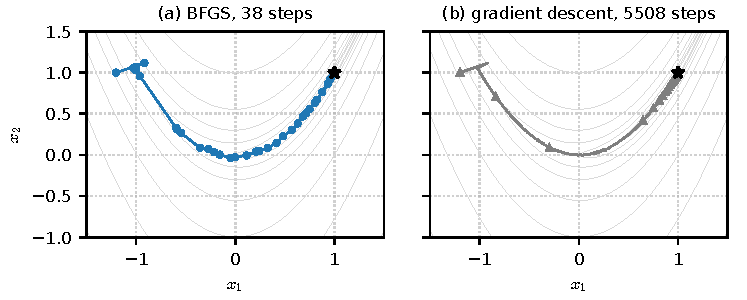
\includegraphics{rosenbrock_path.pdf}
  \caption{The Rosenbrock function from $x_0 = (-1.2, 1)$,
    $\varepsilon = 10^{-6}$: (a)~BFGS, every iterate ($38$ steps);
    (b)~gradient descent, a marker at every 100th of its $5508$
    iterates. The star is ${x^* = (1, 1)}$.}
  \label{fig:path}
\end{figure}

Every accepted step of the three methods satisfies~\eqref{eq:armijo}
and~\eqref{eq:wolfe} and has $s_k^\T y_k > 0$, so by
Theorem~\ref{thm:bfgs} every BFGS matrix stays positive definite. Over
the BFGS steps,
$(f(x_k) - f(x_{k+1})) / (\alpha_k \lvert g_k^\T p_k \rvert) \geq 0.181
\geq c_1$,
$\lvert g_{k+1}^\T p_k \rvert / \lvert g_k^\T p_k \rvert \leq 0.876
\leq c_2$ and $s_k^\T y_k \geq 5.5 \cdot 10^{-9}$. BFGS takes the unit
step in its last $10$ iterations, and its last matrix, rounded to four
decimals, is close to the inverse Hessian at $x^*$:
\[
  H_k = \begin{pmatrix} 0.5 & 1 \\ 1 & 2.0051 \end{pmatrix}, \qquad
  \grad^2 f(x^*)^{-1} = \begin{pmatrix} 0.5 & 1 \\ 1 & 2.005 \end{pmatrix}.
\]

With $\varepsilon = 10^{-12}$, all three methods reach the test without
stalling: gradient descent in $18168$ iterations, BFGS and L-BFGS in
$40$. The error ratios $e_{k+1}/e_k$ of BFGS and L-BFGS
(Figure~\ref{fig:rates}) stay near $1$ for most iterations, then fall
toward $0$, not monotonically; the geometric means of their last four
are $0.0095$ and $0.0143$. Theorem~\ref{thm:lbfgs} promises L-BFGS only
an R-linear rate, but here $m = 5$ exceeds $n = 2$, so the stored pairs
span the whole space and L-BFGS can behave almost like BFGS.

The ratios of gradient descent stay near $1$: their geometric mean over
the last $1000$ steps is $0.9990$, close to
$(\kappa - 1)/(\kappa + 1) = 0.9992$, and single ratios scatter around
it, some above. This does not contradict Theorem~\ref{thm:sd}, which
assumes a quadratic, exact line searches and the norm
$\norm{\cdot}_A$, none of which holds here.

\begin{figure}[tbp]
  \centering
  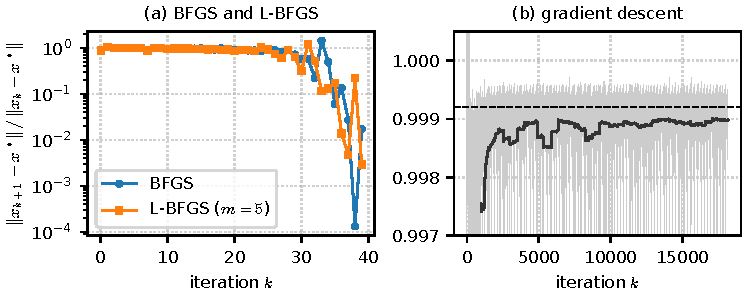
\includegraphics{rosenbrock_rates.pdf}
  \caption{Error ratios $\norm{x_{k+1} - x^*} / \norm{x_k - x^*}$ on
    the Rosenbrock function, $\varepsilon = 10^{-12}$: (a)~BFGS and
    L-BFGS ($m = 5$); (b)~gradient descent: light grey, each ratio;
    solid, the geometric mean of the preceding $1000$ ratios; dashed,
    $(\kappa - 1)/(\kappa + 1) = 0.9992$.}
  \label{fig:rates}
\end{figure}

\subsection{TRIDIA and Raydan~1}\label{sec:vilin}

The pairs save most of the iterations of gradient descent, and neither
quasi-Newton method always needs fewer. TRIDIA and Raydan~1 are two
functions of Vilin~\cite{vilin2018}, the course's MATLAB framework, from
Andrei's collection~\cite{andrei2008}:
\[
  f(x) = (x_1 - 1)^2 + \sum_{i=2}^n i\,(2x_i - x_{i-1})^2
  \quad\text{and}\quad
  f(x) = \sum_{i=1}^n \frac{i}{10}\,\bigl(e^{x_i} - x_i\bigr),
\]
with the minimizers $x^*_i = 2^{1-i}$ and $x^* = 0$. In words, TRIDIA
is a convex quadratic coupling neighboring variables, and Raydan~1 a
weighted sum of convex functions of one variable. Both are uniformly
convex in the sense of Theorem~\ref{thm:global}: TRIDIA has a constant
positive definite Hessian, and the diagonal Hessian $(i/10)\, e^{x_i}$
of Raydan~1 is bounded above and away from $0$ on the level set of
$x_0$, where every $x_i$ stays bounded. So Theorems~\ref{thm:global}
and~\ref{thm:lbfgs} guarantee convergence; we measure its cost at
$n = 100$.

BFGS needs the fewest iterations on TRIDIA and L-BFGS on Raydan~1, both
far fewer than gradient descent (Table~\ref{tab:vilin}). All runs
meet~\eqref{eq:stop}, and BFGS and L-BFGS use only a few more
evaluations than iterations, so their line search nearly always accepts
the first trial step. The two differ only in the memory of five pairs
and in the scaling~\eqref{eq:gamma}, renewed at every iteration; these
runs do not show which difference makes L-BFGS slower on TRIDIA and
faster on Raydan~1.

\begin{table}[tbp]
  \centering\small
  \caption{TRIDIA and Raydan~1, $n = 100$, $x_0 = (1, \dots, 1)$,
    $\varepsilon = 10^{-6}$: iterations, evaluations, and the final
    $\norm{g_k} / \norm{g_0}$.}
  \label{tab:vilin}
  \begin{tabular}{@{}llrrrc@{}}
    \toprule
    function & method & iterations & $f$ evals & $\grad f$ evals
      & $\norm{g_k} / \norm{g_0}$ \\
    \midrule
    TRIDIA   & gradient descent & 2547 & 2655 & 2605 & $9.9 \cdot 10^{-7}$ \\
             & BFGS             &   73 &   79 &   75 & $6.5 \cdot 10^{-7}$ \\
             & L-BFGS ($m = 5$) &  135 &  138 &  137 & $9.2 \cdot 10^{-7}$ \\
    \addlinespace
    Raydan~1 & gradient descent &  220 &  250 &  229 & $9.9 \cdot 10^{-7}$ \\
             & BFGS             &   92 &   93 &   93 & $9.2 \cdot 10^{-7}$ \\
             & L-BFGS ($m = 5$) &   55 &   58 &   57 & $8.9 \cdot 10^{-7}$ \\
    \bottomrule
  \end{tabular}
\end{table}

\subsection{Larger \texorpdfstring{$n$}{n}}\label{sec:large}

L-BFGS keeps the memory and the work of an iteration linear in $n$
while its iteration count grows slowly, so a million variables take
seconds. By Section~\ref{sec:lbfgs}, an L-BFGS iteration needs memory
and work of order $mn$, against $n^2$ for BFGS, and
Theorem~\ref{thm:lbfgs} holds for every $n$. L-BFGS runs at $n = 10^3$
to $10^6$, gradient descent up to $n = 10^5$, capped at $10^4$
iterations, and BFGS only at $n = 10^3$, as a dense $H_k$ needs $8n^2$
bytes and $O(n^2)$ work per iteration.

L-BFGS meets the test at every $n$ (Table~\ref{tab:large}): from
$n = 10^3$ to $10^6$, its iterations grow from $354$ to $1104$ on TRIDIA
and from $121$ to $239$ on Raydan~1, while $n$ grows a thousandfold.
Gradient descent reaches the cap on TRIDIA and needs $983$ to $2159$
iterations on Raydan~1. The time per iteration
(Figure~\ref{fig:scaling}) grows with slope about $2$ for BFGS, the
$O(n^2)$ cost of~\eqref{eq:rank2}, and about $1$ for L-BFGS and gradient
descent (fits to the three largest $n$). In the run reported here, an
iteration of BFGS at $n = 4000$ took tens of milliseconds, longer than
one of L-BFGS at $n = 10^6$, about $10$\,ms, and L-BFGS solved Raydan~1
with $n = 10^6$ in seconds.

\begin{table}[htb]
  \centering\small
  \caption{Iterations from ${x_0 = (1, \dots, 1)}$ to
    meet~\eqref{eq:stop} with ${\varepsilon = 10^{-6}}$. ``cap'': stopped
    at $10^4$ iterations, at $\norm{g_k} / \norm{g_0} = 3.8 \cdot
    10^{-6}$ ($n = 10^3$), $8.5 \cdot 10^{-6}$ ($n = 10^4$) and
    $1.1 \cdot 10^{-5}$ ($n = 10^5$); dash: not run.}
  \label{tab:large}
  \begin{tabular}{@{}llrrrr@{}}
    \toprule
    function & method & $n = 10^3$ & $n = 10^4$ & $n = 10^5$ & $n = 10^6$ \\
    \midrule
    TRIDIA   & gradient descent & cap &  cap &  cap &   -- \\
             & BFGS             & 241 &   -- &   -- &   -- \\
             & L-BFGS ($m = 5$) & 354 &  862 & 1068 & 1104 \\
    \addlinespace
    Raydan~1 & gradient descent & 983 & 1985 & 2159 &   -- \\
             & BFGS             & 249 &   -- &   -- &   -- \\
             & L-BFGS ($m = 5$) & 121 &  214 &  239 &  239 \\
    \bottomrule
  \end{tabular}
\end{table}

\begin{figure}[htb]
  \centering
  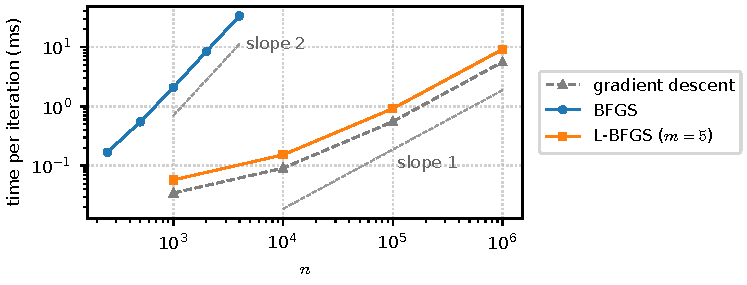
\includegraphics{scaling.pdf}
  \caption{Time per iteration on TRIDIA, in milliseconds, the fastest of
    five runs of $30$ iterations; dashed lines: slopes $1$ and $2$.
    Measured in one execution of the notebook on one loaded machine;
    read only the slopes and orders of magnitude.}
  \label{fig:scaling}
\end{figure}

\subsection{Checks against SciPy}\label{sec:scipy}

SciPy confirms our update to rounding error, and our solvers to the
accuracy of the stopping test. SciPy's BFGS and
L-BFGS-B~\cite{byrd1995}, an L-BFGS method for bound constraints used
here without bounds, are independent codes with their own line
searches; they check~\eqref{eq:bfgs} and our solvers. SciPy's BFGS
takes $32$ iterations on the Rosenbrock function, until
$\norm{g_k} \leq 10^{-5}$. Applying~\eqref{eq:bfgs} along all but its
last step (SciPy does not update after the step that meets its test)
from $H_0 = I$, as SciPy does not scale $H_0$, gives its last matrix to
a relative difference of $3.0 \cdot 10^{-13}$ in the Frobenius norm.

Table~\ref{tab:scipy} compares our BFGS with SciPy's at $n = 100$ and
our L-BFGS with L-BFGS-B at $n = 1000$. SciPy's tolerances are set to
apply~\eqref{eq:stop}, in the max norm for L-BFGS-B, with its test on
the decrease of $f$ switched off ($\code{ftol} = 0$). The iteration
counts differ, since the codes differ in the line search, in $H_0$, the
identity in SciPy's BFGS, and, for L-BFGS-B, in the norm of the test.

The final points agree to within $6.2 \cdot 10^{-5}$ at $n = 100$ and
$3.7 \cdot 10^{-3}$ at $n = 1000$ in the max norm. That is the accuracy
the test allows: \eqref{eq:stop} is relative to $\norm{g_0}$, and at
$n = 1000$ it already accepts our points at $7.6 \cdot 10^{-4}$ and
$1.3 \cdot 10^{-3}$ from $x^*$, so two codes that both pass it can
differ by about $10^{-3}$.

\begin{table}[htb]
  \centering\small
  \caption{Our methods against SciPy's from $x_0 = (1, \dots, 1)$, all
    stopped by~\eqref{eq:stop} with $\varepsilon = 10^{-6}$ (in the max
    norm for L-BFGS-B); final points $x_{\mathrm{ours}}$ and
    $x_{\mathrm{SciPy}}$.}
  \label{tab:scipy}
  \begin{tabular}{@{}lrrcc@{}}
    \toprule
    & \multicolumn{2}{c}{iterations} & & \\
    \cmidrule(lr){2-3}
    function & ours & SciPy
      & $\norm{x_{\mathrm{ours}} - x_{\mathrm{SciPy}}}_\infty$
      & $\norm{x_{\mathrm{ours}} - x^*}_\infty$ \\
    \midrule
    \multicolumn{5}{@{}l}{\emph{BFGS against SciPy's BFGS, $n = 100$}} \\
    TRIDIA   &  73 & 109 & $6.0 \cdot 10^{-5}$ & $3.7 \cdot 10^{-6}$ \\
    Raydan~1 &  92 &  53 & $6.2 \cdot 10^{-5}$ & $4.6 \cdot 10^{-5}$ \\
    \addlinespace
    \multicolumn{5}{@{}l}{\emph{L-BFGS against SciPy's L-BFGS-B, both
      with $m = 5$, $n = 1000$}} \\
    TRIDIA   & 354 & 335 & $3.7 \cdot 10^{-3}$ & $7.6 \cdot 10^{-4}$ \\
    Raydan~1 & 121 & 136 & $1.1 \cdot 10^{-3}$ & $1.3 \cdot 10^{-3}$ \\
    \bottomrule
  \end{tabular}
\end{table}

\section{Conclusion}\label{sec:conclusion}

\begin{enumerate}[leftmargin=*, nosep]
\item Every Rosenbrock step satisfies the strong Wolfe conditions with
  $s_k^\T y_k > 0$ (Lemma~\ref{lem:wolfe}); BFGS needs $38$ iterations,
  with error ratios falling toward zero, gradient descent $5508$.
\item At $n = 100$, BFGS and L-BFGS save most of the iterations of
  gradient descent; BFGS needs fewer on TRIDIA, L-BFGS on Raydan~1.
\item L-BFGS solves both functions at $n = 10^6$, in $1104$ and $239$
  iterations, with a time per iteration about linear in $n$; for dense
  BFGS it is about quadratic, and $H_k$ would need $8$\,TB.
\item SciPy confirms~\eqref{eq:bfgs} to a relative difference of
  $3.0 \cdot 10^{-13}$, and our solvers to the accuracy of the test,
  about $10^{-3}$ at $n = 1000$.
\end{enumerate}

The findings have limits: three test functions, one starting point
each, one memory $m = 5$, and times from one execution on one loaded
machine, meaningful only as slopes and orders of magnitude. The counts
are exact for this code; another line search, $H_0$ or norm in the test
changes them (Section~\ref{sec:scipy}).

\section*{Code availability}

The notebook \nolinkurl{bfgs_project.ipynb}, in the folder
\nolinkurl{project}, implements
Algorithms~\ref{alg:bfgs}--\ref{alg:twoloop} and computes every number,
table and figure in Sections~\ref{sec:example}, \ref{sec:twoloop}
and~\ref{sec:experiments}. It runs on Python~3.14.1 with NumPy~2.5.0,
SciPy~1.18.1 and Matplotlib~3.11.0, pinned in
\nolinkurl{project/requirements.txt}; with these in a virtual
environment \nolinkurl{project/.venv}, the commands
\begin{center}\scriptsize
\begin{tabular}{@{}l@{}}
  \code{cd project}\\
  \code{.venv/bin/jupyter nbconvert -{}-to notebook -{}-execute
    -{}-inplace bfgs\_project.ipynb}
\end{tabular}
\end{center}
run it; the run reported here took less than a minute. The public
repository \url{https://github.com/innicoder/bfgs-seminar} holds this
paper, its LaTeX source, the notebook with its outputs, and the figures.

\printbibliography

\end{document}
